% !TEX root = ./busty_transcription.tex
\section{Bayesian inference}
\label{sec:bayesian}

\subsection{The problem of parameter inference}

One could argue that the whole goal of formulating theoretical models about
nature is to sharpen our understanding from qualitative statements to precise
quantitative assertions about the relevant features of the natural phenomena in
question \cite{Gunawardena2014}. It is in these models that we intend to distill
the essential parts of the object of study. Writing down such models leads to a
propagation of mathematical variables that parametrize our models. By assigning
numerical values to these parameters we can compute concrete predictions that
can be contrasted with experimental data. For these predictions to match the
data the parameter values have to carefully be chosen from the whole parameter
space. But how do we go about assessing the effectiveness of different regions
of parameter space to speak to the ability of our model to reproduce the
experimental observations? The language of probability, and more specifically of
Bayesian statistics is -- we think -- the natural language to tackle this
question.

\subsubsection{Bayes' theorem}

Bayes' theorem is a simple mathematical statement that can apply to \textit{any}
logical conjecture. For two particular events $A$ and $B$ that potentially 
depend on each other Bayes' theorem gives us a recipe for how to update our 
beliefs about one, let us say $B$, given some state of knowledge, or lack thereof, about
$A$. In its most classic form Bayes' theorem is written as
\begin{equation}
P(B \mid A) = {P(A \mid B) P(B) \over P(A)},
\end{equation}
where the vertical line $\mid$ is read as ``given that''. So $P(B \mid A)$ is
read as probability of $B$ given that $A$ took place. $A$ and $B$ can be any
logical assertion. In particular the problem of Bayesian inference focuses on
the question of finding the probability distribution of a particular parameter
value given the data.

For a given model with a set of parameters $\vec{\theta} = (\theta_1, \theta_2,
\ldots, \theta_n)$, the so-called \textit{posterior distribution} 
$P(\vec{\theta} \mid D)$, where $D$ is the experimental data, quantifies the
plausibility of a set of parameter values given our observation of some
particular dataset. In other words, through the application of Bayes' formula we
update our beliefs on the possible values that parameters can take upon learning
the outcome of a particular experiment. We specify the word ``update'' as we
come to every inference problem with prior information about the plausibility of
particular regions of parameter space even before performing any experiment.
Even when we claim as researchers that we are totally ignorant about the values
that the parameters in our models can take, we always come to a problem with
domain expertise that can be exploited. If this was not the case, it is likely
that the formulation of our model is not going to capture the phenomena we claim
to want to understand. This prior information is captured in the \textit{prior
probability} $P(\vec{\theta})$. The relationship between how parameter values
can connect with the data is enconded in the \textit{likelihood function} $P(D
\mid \vec{\theta})$. Our theoretical model, whether deterministic or
probabilistic, is encoded in this term that can be intuitively understood as the
probability of having observed the particular experimental data we have at hand
given that our model is parametrized with the concrete values $\vec{\theta}$. 
Implicitly here we are also conditioning on the fact that our theoretical model
is ``true,'' i.e. the model itself if evaluated or simulated in the computer is
capable of generating equivalent datasets to the one we got to observe in an 
experiment. In this way Bayesian inference consists of applying Bayes' formula 
as 
\begin{equation}
P(\vec{\theta} \mid D) \propto P(D \mid \vec{\theta}) P(\vec{\theta}).
\end{equation}
Notice than rather than writing the full form of Bayes' theorem, we limit 
ourselves to the terms that depend on our quantity of interest -- that is the 
parameter values themselves $\vec{\theta}$ -- as the denominator $P(D)$ only
serves as a normalization constant.

We also emphasize that the dichotomy we have presented between prior and
likelihood is more subtle. Although it is often stated that our prior
knowledge is entirely encapsulated by the obviously named prior
probability $P(\vec{\theta})$, this is usually too simplistic.
The form(s) we choose for our likelihood function
$P(D \mid \vec{\theta})$ also draw heavily on our prior domain expertise
and the assumptions, implicit and explicit, that these choices encode are
at least as important, and often inseparable from,
the prior probability, as persuasively argued in~\cite{Gelman2017}.

\subsubsection{The likelihood function}

As we alluded in the previous section it is through the likelihood function 
$P(D \mid \vec{\theta})$ that we encode the connection between our parameter 
values and the experimental observables. Broadly speaking there are two classes
of models that we might need to encode into our likelihood function:
\begin{itemize}
        \item Deterministic models: Models for which a concrete selection of
        parameter values give a single output. Said differently, models 
        with a one-to-one mapping between inputs and outputs.
        \item Probabilistic models: As the name suggests, models that, rather than
        having a one-to-one input-output mapping, describe the full
        probability distribution of possible outputs.
\end{itemize}
In this paper we focus on inference done with probabilistic models. After all,
the chemical master equations we wrote down describe the time evolutions of the
mRNA probability distribution. So all our terms $P(\vec{\theta} \mid D)$ will be
given by the steady-state solution of the corresponding chemical master equation
in question. This is rather convenient as we do not have to worry about adding a
statistical model on top of our model to describe deviations from the
predictions. Instead our models themselves focus on predicting such variation
in cell count.

\subsubsection{Prior selection}
The different models explored in this work embraced different levels of
coarse-graining that resulted in a diverse number of parameters for different
models. For each of these model configurations Bayes' theorem demands from us to
represent our preconceptions on the possible parameter values in the form of the
prior $P(\vec{\theta})$. Throughout this work for models with $> 1$ parameter we
assign independent priors to each of the parameters; this is
\begin{equation}
P(\vec{\theta}) = \prod_{i=1}^n P(\theta_i).
\end{equation}
Although it is not uncommon practice to use non-informative, or maximally
uninformative priors, we are of the mindset that this is a disservice to the
philosophical and practical implications of Bayes' theorem. It sounds almost
contradictory to claim that can we represent our thinking about a natural
phenomenon in the form of a mathematical model -- in the context of Bayesian
inference this means choosing a form for the likehihoods, and even making
this choice presupposes prior understanding or assumptions as to the
relevant features in the system under study -- but that we have absolutely
no idea what the parameter values could or could not be. We therefore make
use of our own expertise, many times in the form of order-of-magnitude
estimates, to write down weakly-informative prior distributions
for our parameters.

For our particular case all of the datasets from~\cite{Jones2014} used in this
paper have $\mathcal{O}(10^3)$ data points. What this implies is that our
particular choice of priors will not significantly affect our inference as long
as they are broad enough. A way to see why this is the case is to simply look at
Bayes' theorem. For $N ~ 1000-3000$ datum all of the independent of each other
and $n \ll 10^3$ parameters Bayes' theorem reads as
\begin{equation}
P(\vec{\theta} \mid D) \propto \prod_{k=1}^{N} P(d_k \mid \vec{\theta})
\prod_{i=1}^n P(\theta_i),
\end{equation}
where $d_k$ represents the $k$-th datum. That means that if our priors span a
wide range of parameter space, the posterior distribution would be dominated by
the likelihood function.

\subsubsection{Expectations and marginalizations}
For models with more than one or two parameters, it is generally difficult
to visualize or reason about the full joint posterior distribution
$P(\vec{\theta} \mid D)$ directly.
One of the great powers of Bayesian analysis is \textit{marginalization},
allowing us to reduce the dimensionality to only the parameters of
immediate interest by averaging over the other dimensions.
Formally, for a three dimensional model with parameters
$\theta_1$, $\theta_2$, and $\theta_3$, we can for instance
marginalize away $\theta_3$ to produce a 2D posterior as
\begin{equation}
P(\theta_1, \theta_2 \mid D) \propto
        \int_{\theta_3} d\theta_3 \,P(\theta_1, \theta_2, \theta_3 \mid D),
\end{equation}
or we can marginalize away $\theta_1$ and $\theta_3$ to produce the
1D marginal posterior of $\theta_2$ alone, which would be
\begin{equation}
P(\theta_2 \mid D) \propto
        \int_{\theta_1} d\theta_1 \int_{\theta_3} d\theta_3
        \,P(\theta_1, \theta_2, \theta_3 \mid D).
\end{equation}
Conceptually, this is what we did in generating the 2D slices of the
full 9D model in Figure~\ref{fig4:repressed_post_full}(A).
In practice, this marginalization is even easier with Markov Chain Monte Carlo
samples in hand. Since each point is simply a list of parameter values,
we simply ignore the parameters which we want to marginalize
away~\cite{Gelman2013}.
        
\subsubsection{Markov Chain Monte Carlo}
The theory and practice of Bayesian inference with Markov Chain Monte Carlo
(MCMC) is a rich subject with fascinating and deep analogies to statistical
mechanics, even drawing on classical Hamiltonian mechanics and general
relativity in its modern incarnations. We refer the interested reader
to~\cite{Gelman2013} and~\cite{Betancourt2018} for excellent introductions.
Here we merely give a brief summary of
the MCMC computations carried out in this work.

We used the Python package \texttt{emcee} for most of the MCMC sampling
in this work. For the constitutive promoter inference, we also ran
sampling with the excellent Stan modeling language as a check. We did not
use Stan for the inference of the simple repression model because
implementing the gradients of the hypergeometric function ${_2F_1}$
appearing in Eq.~\ref{eq:p_m_bursty+rep_appdx}, the probability
distribution for our bursty model with repression, would have been
an immensely challenging task. \texttt{emcee} was more than adequate for
our purposes, and we were perhaps lucky that the 9-D posterior model
for the model of simple repression with bursty promoter was quite well
behaved and did not require the extra power of the Hamiltonian Monte
Carlo algorithm provided by Stan~\cite{Carpenter2017}.
Source code for all statistical inference will be made available at
\url{https://github.com/RPGroup-PBoC/bursty_transcription}.

\subsection{Bayesian inference on constitutive promoters}
\label{sec:si_bayes_unreg}

Having introduced the ideas behind Bayesian inference we are ready to apply the
theoretical machinery to our non-equilibrium models. In particular in this
section we will focus on model 1 and model 5 in
Figure~\ref{fig2:constit_cartoons}(A). Model 1, the Poisson promoter, will help
us build practical intuition into the implementation of the Bayesian inference
pipeline as we noted in Section~\ref{sec:beyond_means} of the main text that
this model cannot be reconciled with experimental data from observables such as
the Fano factor. In other words, we acknowledge that this model is ``wrong,''
but we still see value in going through the analysis since the simple nature of
the model translates into a neat statistical analysis.

\subsubsection{Model 1 - Poisson promoter}

As specified in the main test, the mRNA steady-state distribution for model 1 in
Figure~\ref{fig2:constit_cartoons}(A) is Poisson with parameter $\lambda$.
Throughout this Appendix we will appeal to the convenient notation for
probability distributions of the form
\begin{equation}
m \sim \text{Poisson}(\lambda),
\end{equation}
where the simbol ``$\sim$'' can be read as \textit{is distributed according to}.
So the previous equation can be read as: the mRNA copy number $m$ is distributed
according to a Poisson distribution with parameter $\lambda$. Our objective then
is to compute the posterior probability distribution $P(\lambda \mid D)$, where,
as in the main text, $D = \{ m_1, m_2, \ldots, m_N \}$ are the data consisting
of single-cell mRNA counts. Since we can assume that each of the cells mRNA
counts are independent of any other cells, our likelihood function $P(D \mid
\lambda)$ consists of the product of $N$ Poisson distributions.

To proceed with the inference problem we need to specify a prior. In this case
we are extremely data-rich, as the dataset from Jones et.\ al~\cite{Jones2014}
has of order 1000-3000 single-cell measurements for each promoter, so our choice
of prior matters little here, as long as it is sufficiently broad. A convenient
choice for our problem is to use a \textit{conjugate} prior. A conjugate prior
is a special prior that causes the posterior to have the same functional form as
the prior, simply with updated model parameters. This makes calculations
analytically tractable and also offers a nice interpretation of the inference
procedure as updating our knowledge about the model parameters. This makes
conjugate priors very useful when they exist. The caveat is that conjugate
priors only exist for a very limited number of likelihoods, mostly with only one
or two model parameters, so in almost all other Bayesian inference problems, we
must tackle the posterior numerically.

But, for the problem at hand, a conjugate prior does in fact exist. For a
Poisson likelihood of identical and identically distributed data, the conjugate
prior is a gamma distribution, as can be looked up in, e.g.,~\cite{Gelman2013},
Section 2.6. Putting a gamma prior on $\lambda$ introduces two new parameters
$\alpha$ and $\beta$ which parametrize the gamma distribution itself, which we
use to encode the range of $\lambda$ values we view as reasonable. Recall
$\lambda$ is the mean steady-state mRNA count per cell, which \textit{a priori}
could plausibly be anywhere from 0 to a few hundred. $\alpha=1$ and $\beta=1/50$
achieve this, since the gamma distribution is strictly positive with mean
$\alpha/\beta$ and standard deviation $\sqrt{\alpha}/\beta$. To be explicit,
then, our prior is
\begin{equation}
\lambda \sim \text{Gamma}(\alpha, \beta)
\end{equation}

As an aside, note that if we did not know that our prior was a conjugate prior,
we could still write down our posterior distribution from its definition as
\begin{equation}
p(\lambda\mid D,\alpha,\beta)
\propto p(D\mid\lambda) p(\lambda \mid\alpha,\beta)
\propto \left(\prod_{k=1}^N \frac{\lambda^{m_k}e^{-\lambda}}{m_k!}\right)
        \frac{\beta}{\Gamma(\alpha)}(\beta\lambda)^{\alpha-1} e^{-\beta\lambda}
.
\end{equation}
Without foreknowledge that this in fact reduces to a gamma distribution, this
expression might appear rather inscrutable. When conjugate priors are
unavailable for the likelihood of interest - which is almost always the case for
models with $>1$ model parameter - this inscrutability is the norm, and making
sense of posteriors analytically is almost always impossible. Fortunately, MCMC
sampling provides us a powerful method of constructing posteriors numerically
which we will make use of extensively.

Since we did use a conjugate prior, we may simply look up our posterior in any
standard reference such as~\cite{Gelman2013}, Section 2.6,
from which we find that
\begin{equation}
\lambda
\sim \text{Gamma}\left(\alpha + \bar{m}N, \beta + N\right),
\end{equation}
where we defined the sample mean $\bar{m} = \frac{1}{N}\sum_k m_k$ for
notational convenience. A glance at the FISH data from~\cite{Jones2014} reveals
that $N$ is $\mathcal{O}(10^3)$ and $\langle m\rangle \gtrsim 0.1$ for all
constitutive strains in~\cite{Jones2014}, so $\bar{m}N \gtrsim 10^2$. Therefore
as we suspected, our prior parameters are completely overwhelmed by the data.
The prior behaves, in a sense, like $\beta$ extra ``data points''
with a mean value of $(\alpha-1)/\beta$~\cite{Gelman2013}, which
gives us some intuition for how much data is needed to overwhelm
the prior in this case: enough data $N$ such that $\beta\ll N$
and $\alpha/\beta \ll \bar{m}$. In
fact, $\bar{m}N$ and $N$ are so large that we can, to an excellent
approximation, ignore the $\alpha$ and $\beta$ dependence and approximate the
gamma distribution as a Gaussian with mean $\bar{m}$ and standard deviation
$\sqrt{\bar{m}/N}$, giving
\begin{equation}
\lambda
\sim \text{Gamma}\left(\alpha + \bar{m}N, \beta + N\right)
\approx \text{Normal}\left(\bar{m}, \sqrt{\frac{\bar{m}}{N}}\right).
\end{equation}
As an example with real numbers, for the \textit{lacUV5} promoter, Jones et.\
al~\cite{Jones2014} measured 2648 cells with an average mRNA count per cell of
$\bar{m} \approx 18.7$. In this case then, our posterior is
\begin{equation}
\lambda
\sim \text{Normal}\left(18.7, 0.08\right),
\label{eq:gauss_posterior}
\end{equation}
which suggests we have inferred our model's one parameter to a precision of
order 1\%.

This is not wrong, but it is not the full story. The model's posterior
distribution is tightly constrained, but is it a good generative model? In other
words, if we use the model to generate synthetic data in the computer does it
generate data that look similar to our actual data, and is it therefore
plausible that the model captures the important features of the data generating
process? This intuitive notion can be codified with \textit{posterior predictive
checks}, or PPCs, and we will see that this simple Poisson model fails badly.

The intuitive idea of posterior predictive checks is simple: 
\begin{enumerate}
\item Make a random draw of the model parameter $\lambda$ from the posterior
distribution.
\item Plug that draw into the likelihood and generate a synthetic dataset
$\{m_k\}$ conditioned on $\lambda$.
\item Repeat many times.
\end{enumerate}
More formally, the posterior predictive distribution can be thought of as the
distribution of future yet-to-be-observed data, conditioned on the data we have
already observed. Clearly if those data appear quite different, the model has a
problem. Put another way, if we suppose the generative model is true, i.e. we
claim that our model explains the process through which our observed
experimental data was generated, then the synthetic datasets we generate should
resemble the actual observed data. If this is not the case, it suggests the
model is missing important features. All the data we consider in this work are
1D (distributions of mRNA counts over a population) so empirical cumulative
distribution functions ECDFs are an excellent visual means of comparing
synthetic and observed datasets. In general for higher dimensional datasets,
much of the challenge is in merely designing good visualizations that can
actually show if synthetic and observed data are similar or not.

For our example Poisson promoter model then, we merely draw many random numbers,
say 1000, from the Gaussian posterior in Eq.~\ref{eq:gauss_posterior}. For each
one of those draws, we generate a dataset from the likelihood, i.e., we draw
2648 (the number of observed cells in the actual dataset) Poisson-distributed
numbers for each of the 1000 posterior draws, for a total of 2648000 samples
from the posterior predictive distribution.

To compare so many samples with the actual observed data, one excellent
visualization for 1D data is ECDFs of the quantiles, as shown for our Poisson
model in~\fig{fig:constit_post_full}(B) in the main text. 

\subsubsection{Model 5 - Bursty promoter}

Let us now consider the problem of parameter inference from FISH data for model
five from~\fig{fig1:means_cartoons}(C). As derived in
Appendix~\ref{sec:gen_fcn_appdx}, the steady-state mRNA distribution in this
model is a negative binomial distribution, given by
\begin{equation}
p(m) = \frac{\Gamma(m+k_i)}{\Gamma(m+1)\Gamma(k_i)}
        \left(\frac{1}{1+b}\right)^{k_i}
        \left(\frac{b}{1+b}\right)^m,
\label{eq:si_neg_bionom}
\end{equation}
where $b$ is the mean burst size and $k_i$ is the burst rate nondimensionalized
by the mRNA degradation rate $\gamma$. As sketched earlier, we can intuitively
think about this distribution through a simple story. The story of this
distribution is that the promoter undergoes geometrically-distributed bursts of
mRNA, where the arrival of bursts is a Poisson process with rate $k_i$ and the
mean size of a burst is $b$.

As for the Poisson promoter model, this expression for the steady-state mRNA
distribution is exactly the likelihood we want to use in Bayes' theorem. Again
denoting the single-cell mRNA count data as $D=\{m_1, m_2,\dots, m_N\}$, here
Bayes' theorem takes the form
\begin{equation}
p(k_i, b \mid D) \propto p(D\mid k_i,b)p(k_i, b),
\end{equation}
where the likelihood $p(D\mid k_i,b)$ is given by the product of $N$ negative
binomials as in Eq.~\ref{eq:si_neg_bionom}. We only need to choose priors on
$k_i$ and $b$. For the datasets from~\cite{Jones2014} that we are analyzing, as
for the Poisson promoter model above we are still data-rich so the prior's
influence remains weak, but not nearly as weak because the dimensionality of our
model has increased from one to two.

We follow the guidance of~\cite{Gelman2013}, Section 2.9 in opting for
weakly-informative priors on $k_i$ and $b$ (conjugate priors do not exist for
this problem), and we find ``street-fighting estimates''~\cite{Mahajan2010} to
be an ideal way of constructing such priors. The idea of weakly informative
priors is to allow all remotely plausible values of model parameters while
excluding the completely absurd or unphysical.

Consider $k_i$. Some of the strongest known bacterial promoters control rRNA
genes and initiate transcripts no faster than $\sim 1/\text{sec}$. It would be
exceedingly strange if any of the constitutive promoters from~\cite{Jones2014}
were stronger than that, so we can take that as an upper bound. For a lower
bound, if transcripts are produced too rarely, there would be nothing to see
with FISH. The datasets for each strain contain of order $10^3$ cells, and if
the $\langle m \rangle = k_i b/\gamma \lesssim 10^{-2}$, then the total number
of expected mRNA detections would be single-digits or less and we would have
essentially no data on which to carry out inference. So assuming $b$ is not too
different from 1, justified next, and an mRNA lifetime of $\gamma^{-1}\sim
3-5~\text{min}$, this gives us soft bounds on $k_i/\gamma$ of perhaps $10^{-2}$
and $3\times 10^1$.

Next consider mean burst size $b$. This parametrization of the geometric
distribution allows bursts of size zero (which could representing aborted
transcripts and initiations), but it would be quite strange for the mean burst
size $b$ to be below $\sim10^{-1}$, for which nearly all bursts would be of size
zero or one. For an upper bound, if transcripts are initiating at a rate
somewhat slower than rRNA promoters, then it would probably take a time
comparable to the lifetime of an mRNA to produce a burst larger than 10-20
transcripts, which would invalidate the approximation of the model that the
duration of bursts are instantaneous compared to other timescales in the
problem. So we will take soft bounds of $10^{-1}$ and $10^1$ for $b$.

Note that the natural scale for these ``street-fighting estimates'' was a log
scale. This is commonly the case that our prior sense of reasonable and
unreasonable parameters is set on a log scale. A natural way to enforce these
soft bounds is therefore to use a lognormal prior distribution, with the soft
bounds set $\pm2$ standard deviations from the mean.

With this, we are ready to write our full generative model as
\begin{equation}
\begin{split}
\ln k_i \sim \text{Normal}(-0.5, 2),
\\
\ln b \sim \text{Normal}(0.5, 1),
\\
m \sim \text{NBinom}(k_i, b).
\end{split}
\end{equation}
Section~\ref{section_04_bayesian_inference} in the main text details the
results of applying this inference to the single-cell mRNA counts data. There
we show the posterior distribution for the two parameters for different 
promoters. Figure~\ref{figS:ppc_unreg} shows the so-called posterior predictive
checks (see main text for explanation) for all 18 unregulated promoters shown
in the main text.

\begin{figure}[p]
\centering
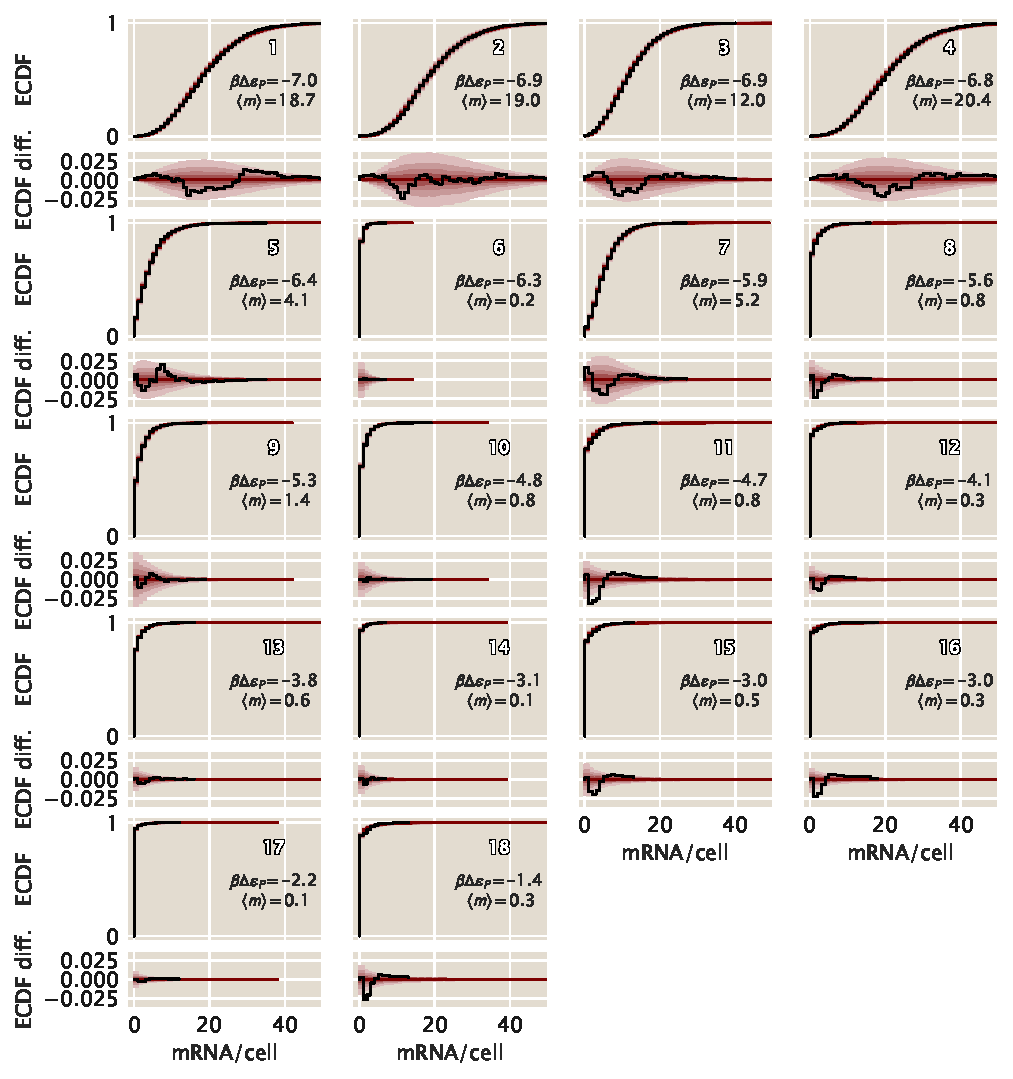
\includegraphics{../../figures/si/figS0X_ppc.pdf}
\caption{\textbf{Theory-data comparison of inference on unregulated promoters.}
Comparison of the inference (red shaded area) vs the experimental measurements
(black lines) for 18 different unregulated promoters with different mean mRNA
expression levels from Ref.~\cite{Jones2014}. Upper panels show the empirical
cumulative distribution function (ECDF), while the lower panels show the
differences with respect to the median of the posterior samples. White numbers
are the same as in Figure~\ref{fig1:means_cartoons} for cross comparison. The
predicted binding energies $\beta\Delta\varepsilon_p$ were obtained from the
energy matrix model in Ref.~\cite{Brewster2012}}
\label{figS:ppc_unreg}
\end{figure}

\subsection{Bayesian inference on the simple-repression architecture}

As detailed in~\ref{section_04_bayesian_inference} in the main text the
inference on the unregulated promoter served as a stepping stone towards our
ultimate goal of inferring repressor rates from the steady-state mRNA
distributions of simple-repression architectures. For this we expand the
one-state bursty promoter model to a two-state promoter as schematized in
Figure~\ref{fig1:means_cartoons}(C) as model 5. This model adds two new
parameters: the repressor binding rate $k^+$, solely function of the repressor
concentration, and the repressor dissociation rate $k^-$, solely a function of
the repressor-DNA binding affinity.

The structure of the data in~\cite{Jones2014} for regulated promoters tuned
these two parameters independently. In their work the production of the LacI
repressor was under the control of an inducible promoter regulated by the TetR
repressor as schematized in Figre~\ref{figS:aTc_circuit}. When TetR binds to the
small molecule anhydrotetracycline (aTc), it shifts to an inactive conformation
unable to bind to the DNA. This translates into an increase in gene expression
level. In other words, the higher the concentration of aTc added to the media,
the less TetR repressors that can control the expression of the \textit{lacI}
gene, so the higher the concentration of LacI repressors in the cell. So by 
tuning the amount of aTc in the media where the experimental strains were grown
they effectively tune $k^+$ in our simple theoretical model. On the other hand
to tune $k^-$ the authors swap three different binding sites for the LacI 
repressor, each with different repressor-DNA binding affinities previously 
characterized \cite{Garcia2011a}.

\begin{figure}[h!]
\centering
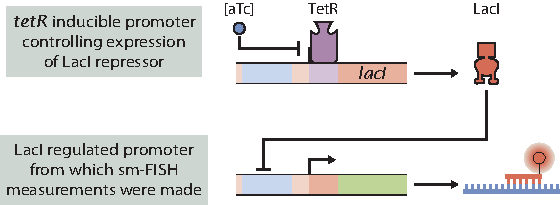
\includegraphics{../../figures/si/figS0X_aTc_circuit.pdf}
\caption{\textbf{aTc controlled expression of LacI repressor.} Schematic of the
circuit used in~\cite{Jones2014} to control the expression of the LacI
repressor. The \textit{lacI} gene is under the control of the TetR repressor. As
the TetR repressor is inactivated upon binding of anhydrotetracycline or aTc,
the more aTc added to the media were cells are growing, the less TetR repressors
available to control the expression of the \textit{lacI} gene, resulting in more
LacI repressors per cell. LacI simultaneously controls the expression of the
mRNA on which single-molecule mRNA FISH was performed for gene expression
quantification.}
\label{figS:aTc_circuit}
\end{figure}

What this means is that we have access to data with different combinations of
$k^-$ and $k^+$. We could naively try to fit the kinetic parameters individually
for each of the datasets, but there is no reason to believe that the binding
site identity for the LacI repressor somehow affects its expression level
controlled from a completely different location in the genome, nor vice versa.
In other words, what makes the most sense it to fit all datasets together to
obtain a single value for each of the association and dissociation rates. What
this means, as described in Section~\ref{section_04_bayesian_inference} of the main text
is that we have a seven dimensional parameter space with four possible
association rates $k^+$ given the four available aTc concentrations, and three
possible dissociation rates $k^-$ given the three different binding sites
available in the dataset.

Formally now, denote the set of seven repressor rates to be inferred as
\begin{equation}
\vect{k} =\{k_{Oid}^-, k_{O1}^-, k_{O2}^-,
k_{0.5}^+, k_{1}^+, k_{2}^+, k_{10}^+\}.
\end{equation}
Note that since the repressor copy numbers are not known directly as explained
before, we label their association rates by the concentration of aTc. Bayes
theorem reads simply
\begin{equation}
p(\vect{k}, k_i, b \mid D)
\propto
p(D \mid\vect{k}, k_i, b) p(\vect{k}, k_i, b),
\end{equation}
where $D$ is the set of all $N$ observed single-cell mRNA counts across the
various conditions. We assume that individual single-cell measurements are
independent so that the likelihood factorizes as
\begin{equation}
p(D \mid\vect{k}, k_i, b)
= \prod_{j=1}^N p(m\mid \vect{k}, k_i, b)
= \prod_{j=1}^N p(m\mid k_j^+, k_j^-, k_i, b)
\end{equation}
where $k_j^\pm$ represent the appropriate binding and unbinding rates for the
$j$-th measured cell. Our likelihood function, previously derived in
Appendix~\ref{sec:gen_fcn_appdx}, is given by the rather complicated result in
Eq.~\ref{eq:p_m_bursty+rep_appdx}, which for completeness we reproduce here as
\begin{equation}
\begin{split}
p(m \mid k_R^+, k_R^-, k_i, b) = & ~\frac{
        \Gamma(\alpha + m)\Gamma(\beta + m)\Gamma(k_R^+ + k_R^-)
        }
        {
        \Gamma(\alpha)\Gamma(\beta)\Gamma(k_R^+ + k_R^- + m)
        }
\frac{b^m}{m!}
\\
&\times {_2F_1}(\alpha+m, \beta+m, k_R^++k_R^-+m; -b).
\end{split}
\label{eq:p_m_bursty+rep_infreprint}
\end{equation}
where $\alpha$ and $\beta$, defined for notational convenience, are
\begin{align}
\begin{split}
\alpha &= \frac{1}{2}
\left(k_i+k_R^-+k_R^+ + \sqrt{(k_i+k_R^-+k_R^+)^2 - 4k_i k_R^-}\right)
\\
\beta &= \frac{1}{2}
\left(k_i+k_R^-+k_R^+ - \sqrt{(k_i+k_R^-+k_R^+)^2 - 4k_i k_R^-}\right).
\end{split}
\end{align}

Next we specify priors. As for the constitutive model, weakly informative
lognormal priors are a natural choice for all our rates. We found that if the
priors were too weak, our MCMC sampler would often become stuck in regions of
parameter space with very low probability density, unable to move. We struck a
balance in choosing our prior widths between helping the sampler run while
simultaneously verifying that the marginal posteriors for each parameter were
not artificially constrained or distorted by the presence of the prior. The only
exception to this is the highly informative priors we placed on $k_i$ and $b$,
since we have strong knowledge of them from our inference of constitutive
promoters above.

With priors and likelihood specified we may write down our complete generative model as
\begin{equation}
\begin{split}
\log_{10}k_i &\sim \text{Normal}(0.725, 0.025)\\
\log_{10}b   &\sim \text{Normal}(0.55, 0.025)\\
\log_{10}k_{0.5}^+ &\sim \text{Normal}(-0.45, 0.3)\\
\log_{10}k_{1}^+   &\sim \text{Normal}(0.6, 0.3)\\
\log_{10}k_{2}^+   &\sim \text{Normal}(1.15, 0.3)\\
\log_{10}k_{10}^+  &\sim \text{Normal}(1.5, 0.3)\\
\log_{10}k_{Oid}^- &\sim \text{Normal}(-0.25, 0.3)\\
\log_{10}k_{O1}^-  &\sim \text{Normal}(0.1, 0.3)\\
\log_{10}k_{O2}^-  &\sim \text{Normal}(0.45, 0.3)\\
m &\sim \text{Likelihood}(k_R^+, k_R^-, k_i, b),
\end{split}
\end{equation}
where the likelihood is specified by Eq.~\ref{eq:p_m_bursty+rep_infreprint}.
We ran MCMC sampling on the full nine dimensional posterior specified
by this generative model.

We found that fitting a single operator/aTc concentration at a time with a
single binding and unbinding rate did not yield a stable inference for most of
the possible operator/aTc combinations. In other words, a single dataset could
not independently resolve the binding and unbinding rates, only their ratio as
set by the mean fold-change in Figure~\ref{fig1:means_cartoons} in the main
text. Only by making the assumption of a single unique binding rate for each
repressor copy number and a single unique unbinding rate for each binding site,
as done in Figure~\ref{fig4:repressed_post_full}(A), was it possible to
independently resolve the rates and not merely their ratios.

We also note that we found it necessary to exclude the very weakly and very
strongly repressed datasets from Jones et.\ al.~\cite{Jones2014}. In both cases
there was, in a sense, not enough information in the distributions for our
inference algorithm to extract, and their inclusion simply caused problems for
the MCMC sampler without yielding any new insight. For the strongly repressed
data (Oid, 10~ng/mL aTc), with $>$ 95\% of cells with zero mRNA, there was quite
literally very little data from which to infer rates. And the weakly repressed
data, all with the repressor binding site O3, had an unbinding rate so fast that
the sampler essentially sampled from the prior; the likelihood had negligible
influence, meaning the data was not informing the sampler in any meaningful way,
so no inference was possible.

As suggested by one of our reviewers, in order for readers to judge the
agreement between our predictions and the experimental data for the regulated
case, we include Figure~\ref{figS:reg_histograms} that plot the same data as
Figure~\ref{fig4:repressed_post_full}(C), but rather than showing ECDF, we show
histograms of the individual distributions.

\begin{figure}[p]
\centering
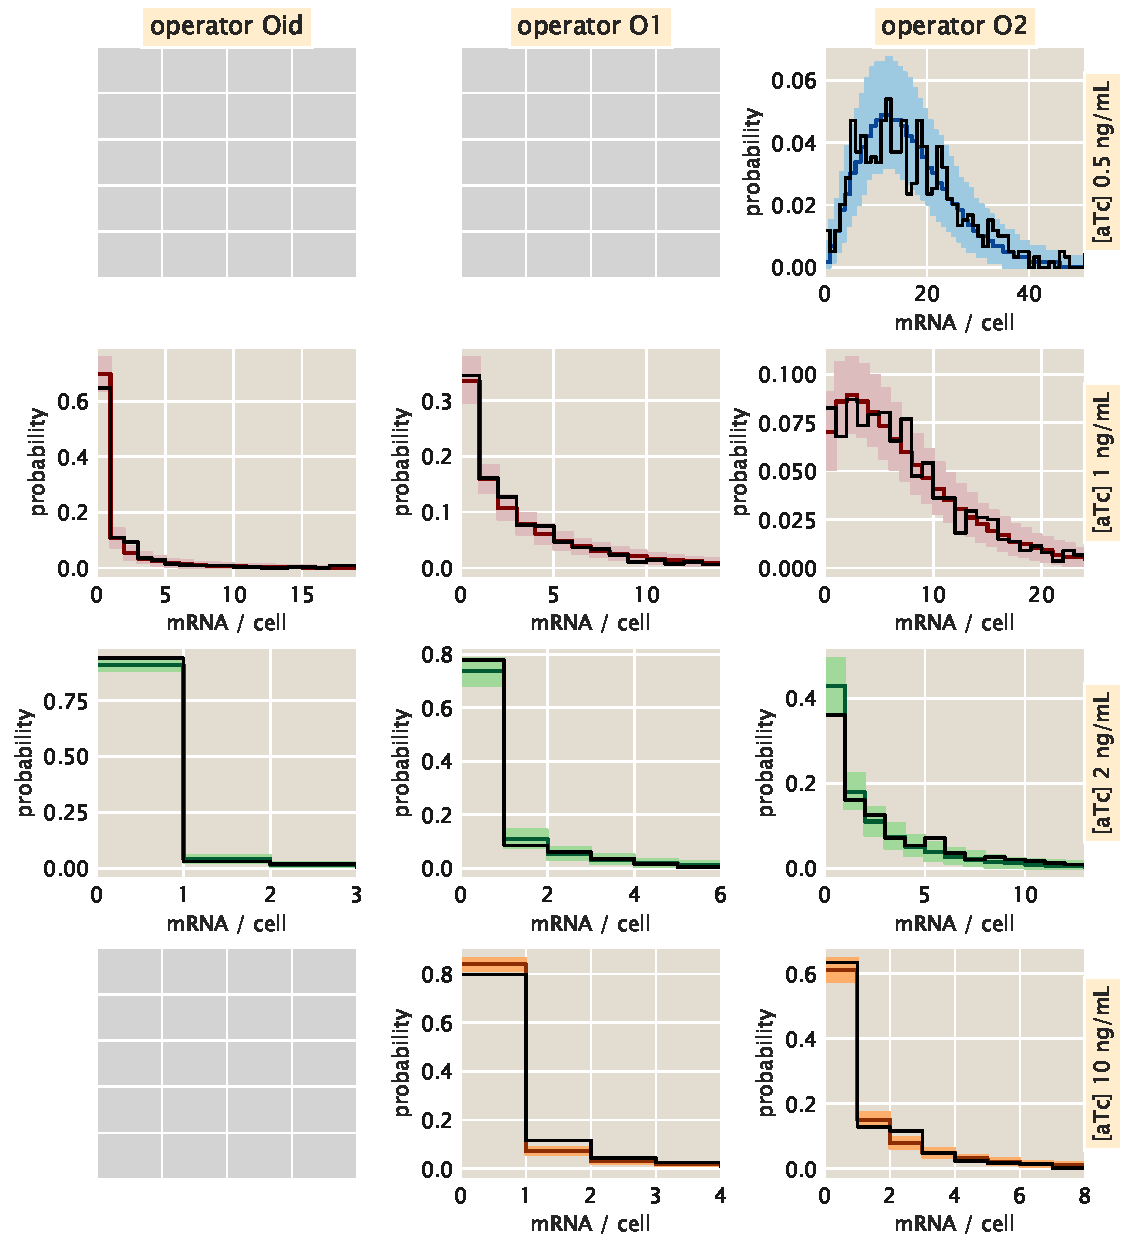
\includegraphics[width=\textwidth]{../../figures/si/figS0X_histograms.pdf}
\caption{\textbf{Theory-experiment comparision of mRNA distributions for
regulated promoters.} Comparison of the inference (color shaded area
encloses the 95\% of all posterior predictive check samples while the color
solid line represents the median of all samples) vs the experimental
measurements (black lines) for different regulated promoters with different
operators (columns) and aTc concentrations (rows) from
Ref.~\cite{Jones2014}.}
\label{figS:reg_histograms}
\end{figure}